%! Author = adnansiddiquei
%! Date = 19/03/2024

\section{Training the model}\label{sec:q1bc}
\begin{figure}[t]
    \centering
    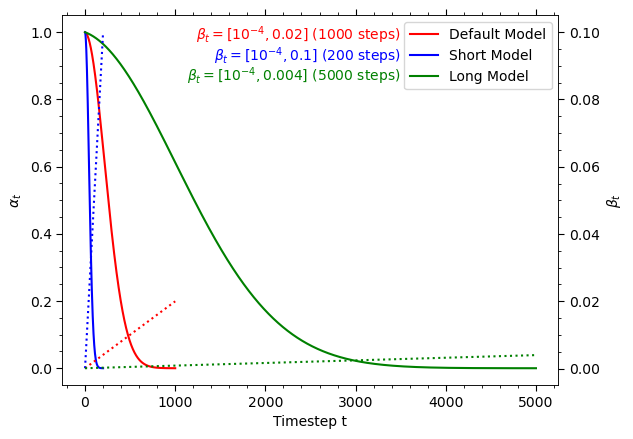
\includegraphics[width=0.8\textwidth]{figures/q1b_noise_schedules}
    \caption{A plot of each noise schedule that was evaluated.
        The dotted lines represent the $\beta_{t}$ values and the solid lines represent the $\alpha_t$ values.}
    \label{fig:q1b_noise_schedules}
\end{figure}
\begin{figure}[t]
    \centering
    \includegraphics[width=0.8\textwidth]{}
    \caption{}
    \label{}
\end{figure}

This section discusses the training of the DDPM model with varying linear noise schedules.

Three different models were trained, the first model (default model) was trained with the provided noise schedule:
$\beta_{t} = [10^{-4}, 0.02]$ with 1000 steps; the second model (the "long model") was trained with a longer noise schedule:
$\beta_{t} = [10^{-4}, 0.004]$ with 5000 steps which added less noise at each step; and the third model (the "short model")
was trained with a shorter noise schedule: $\beta_{t} = [10^{-4}, 0.1]$ with 200 steps which added more noise at each step.
The number of steps was amended for each model such that the final noise level was the same for each model ($\alpha_{t}$
of the order of $10^{-5}$ at the final time step).
Figure~\eqref{fig:q1b_noise_schedules} illustrates the noise schedules used for each model and
